\chapter{电解与极化作用}
% 第十章作业 8 9 10 11 13 16
% 
\begin{itemize}
    \item 可逆电极:平衡,$I \to 0$,无限时间,$\phi_{\mbox{可逆}}$
    \item 不可逆电极:不平衡,$I \neq 0$,不可逆的电极过程,有限时间,$\phi_{\mbox{不可可逆}}$
\end{itemize}


本章主要研究:不可逆电极的电极作用、电解时的真正的充放电效应。


\section{分解电压}

分解电压,指使电解质在电极上分解生成电解产物所需施加的最小电压。电解质的分解电压由其电解产物组成的元电池电动势,阴阳二电极的极化过电位和电路压降三部分组成。

\begin{align*}
    E_{\mbox{分解}} &= E_{\mbox{可逆}} \\ 
    E_{\mbox{分解}} &= E_{\mbox{不可逆}} + \Delta E + IR \\ 
\end{align*}



\section{极化作用}


不可逆电极过程中$\phi$偏离平衡位置的现象。

产生极化的原因:当$I \neq 0$时,电极上发生一系列以一定速率进行的过程。每个过程均有阻力,克服阻力需要推动力,就表现为$\phi$的偏离行为。电池极化分为:

\subsection{浓差极化}

由于浓差扩散过程中存在阻力,使得电极附近的溶液与浓度的本体不同,从而使$\phi$值与平衡值产生一定的偏离。

\subsection{电化学极化}


电极反应的某一步反应速率比较慢,需要比较高的活化能。


极化作用结果总是阴极电极电势下降,阳极电极电势上升。



\section{超电势}


某一电流密度下,实际发生电解的电极电势$\phi$和可逆电极$\phi_0$之间的差距称为超电势。

\subsection{极化曲线}


在给定电流$i$下,电池或电解池中阴极和阳极的实际电极电势的值称为极化曲线。总体上看由于极化的存在不利于能量的利用。

\begin{figure}[h]
    \centering
    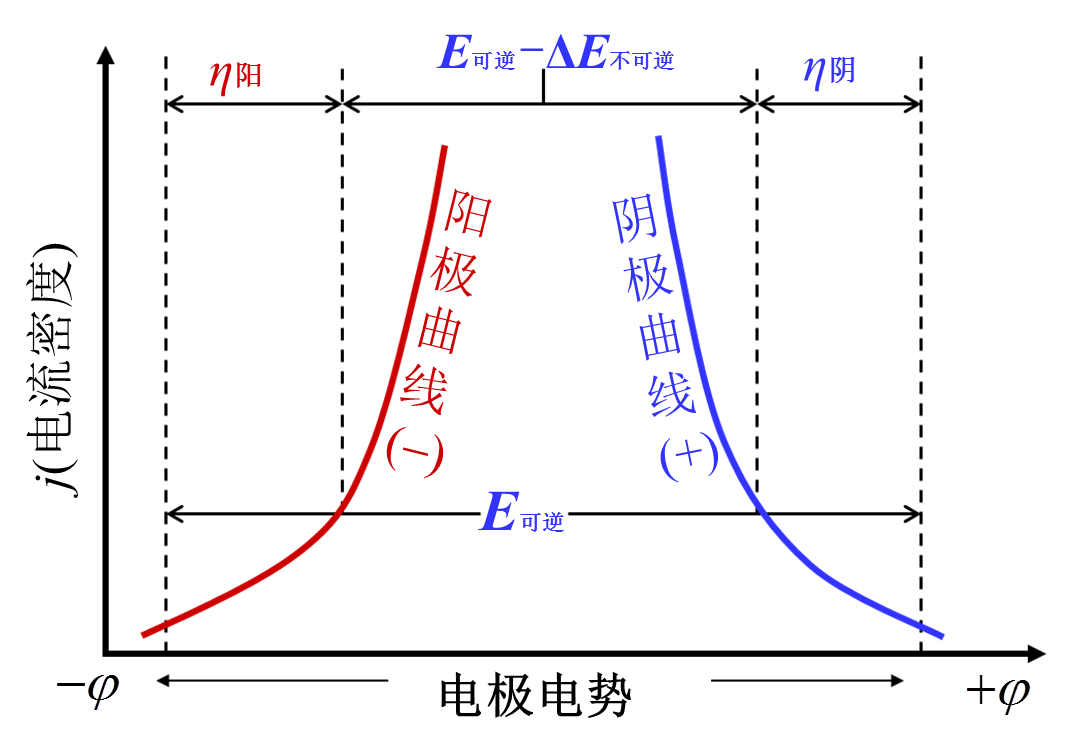
\includegraphics[width=0.7\textwidth]{battery_dmii.png}
    \caption{电池的极化曲线}
    \label{fig:battery_dmii}
\end{figure}

\begin{figure}[h]
    \centering
    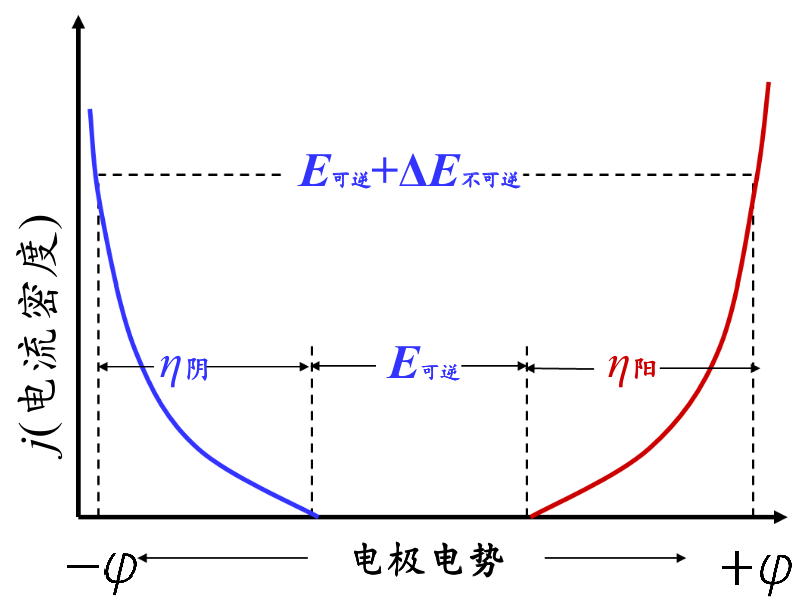
\includegraphics[width=0.7\textwidth]{cell_dmjpii.png}
    \caption{电解池的极化曲线}
    \label{fig:cell_dmjpii}
\end{figure}




\subsection{氢超电势}

电解质溶液通常用水作溶剂,在电解过程中,$\ce{H+}$在阴极会与金属离子竞争还原。
利用氢在电极上的超电势,可以使比氢活泼的金
属先在阴极析出,这在电镀工业上是很重要的。
例如,只有控制溶液的 pH ,利用氢气的析出有
超电势,才使得镀 Zn , Sn , Ni , Cr 等工艺成为现

Tafel, et al. (2007) 提出了一种新的超电势模型,其中氢超电势为

\begin{equation*}
    \eta = a + b \ln \frac{j}{[j]}
\end{equation*}



\section{电解时电极上的竞争反应}


析出电势(不可逆电极电势):电解液中每一种离子析出的时候对应的一个电势。

例如,$\ce{H+}$析出$\ce{H2}$,此时$\phi_{\mbox{不可逆}}$被称为$\ce{H+}$的析出电势。

离子在电极上的析出顺序(即电极反应的确定)

\begin{enumerate}
    \item 阴极上,电势较大,先析出
    \item 阳极上,电势较小,先析出
\end{enumerate}

这一结论的来源可以简单认为,阴极发生的是还原反应,那么还原性越强的离子,电势越大,先析出。
阳极发生的是氧化反应,那么氧化性越强的离子,电势越小,先析出。

\subsection{阴极上发生的化学反应}

电解时在阴极上发生还原反应,发生还原反应的物质通常有:


\subsubsection{金属离子}

\begin{equation*}
    \ce{M^z+}(a)+ z\ce{e-} -> \ce{M}(s)
\end{equation*}

\begin{equation*}
    \phi_{\ce{M | M^z+}} = \phi_{\ce{M | M^z+}}^\ominus - \frac{RT}{zF} Q
\end{equation*}

\subsubsection{氢离子}

\begin{equation*}
    \ce{2H^+}(a)+ 2\ce{e-} -> \ce{H2}(p^\ominus)
\end{equation*}


\begin{equation*}
    \phi_{\ce{H2 | 2H^+}} = \phi_{\ce{H2 | H^+}}^\ominus - \frac{RT}{2F} Q
\end{equation*}

\subsection{阳极上发生的化学反应}

电解时阳极上发生氧化反应,发生氧化反应的物质通常有:

\subsubsection{阴离子}

\begin{equation*}
    \ce{Cl-}(a) \ce{->} \ce{Cl2}(p^\ominus) + 2\ce{e-}
\end{equation*}


\begin{equation*}
    2\ce{OH-}(a) \ce{->} \ce{H2O}(p^\ominus) + 2\ce{e-} + \ce{O2}(p^\ominus)
\end{equation*}


\subsubsection{阳极本身的氧化}

\begin{equation*}
    \ce{Cu(s) -> Cu^2+(a) + 2e-}
\end{equation*}


在阳极\textbf{电极电势最小的}首先在阳极上发生的氧化反应。


\section{金属的电化学腐蚀}


